\documentclass[10pt]{article}
\usepackage[T1]{fontenc}\usepackage[utf8]{inputenc}\usepackage{lmodern}\usepackage{amsmath}\usepackage{xcolor}\usepackage{tikz}\usepackage[paperwidth=18cm,paperheight=20cm,margin=0.5cm]{geometry}\pagestyle{empty}
\begin{document}\noindent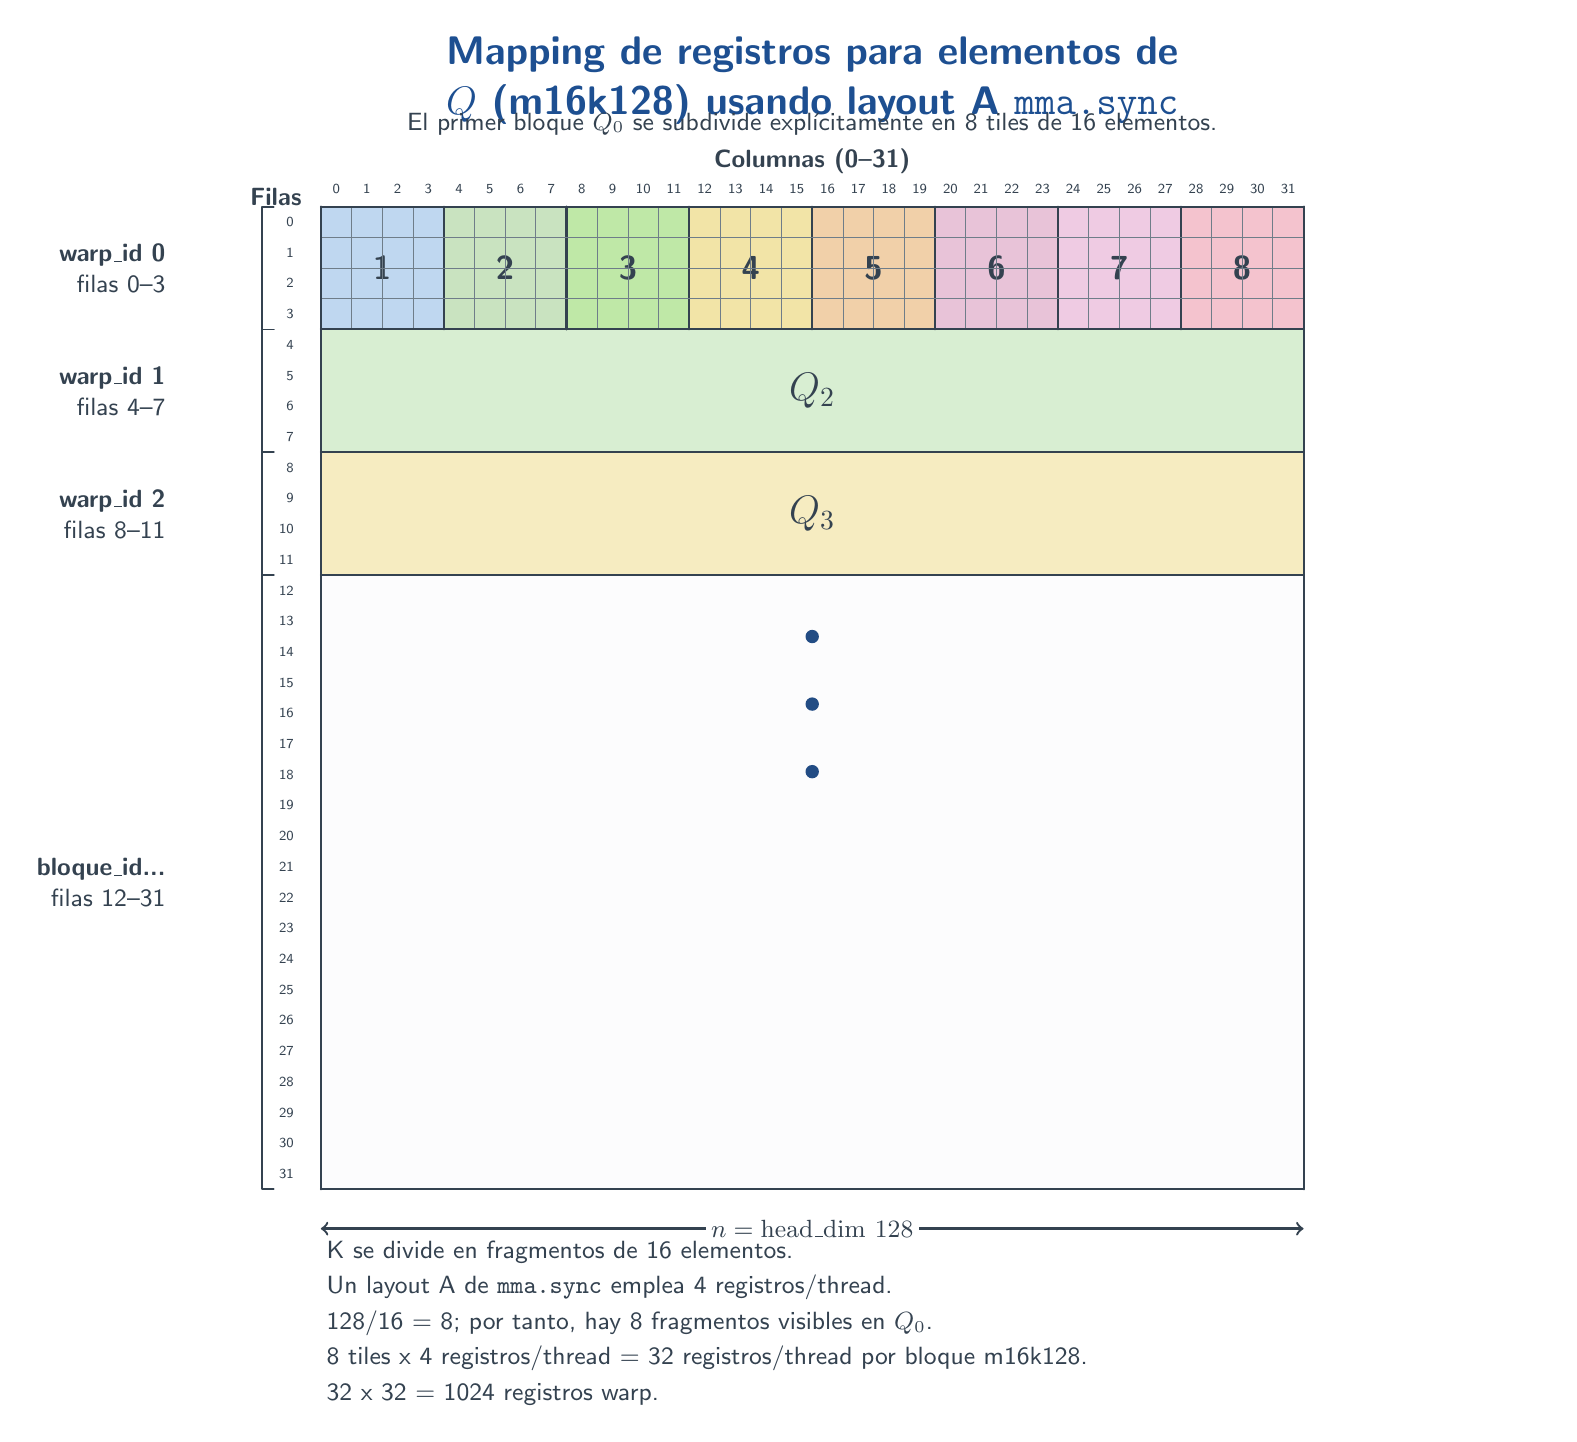
\begin{tikzpicture}[x=1cm,y=1cm,line cap=round,line join=round]
\definecolor{TitleColor}{HTML}{1D4F91}
\definecolor{Grid}{HTML}{6F7D89}
\definecolor{Heavy}{HTML}{344250}
\definecolor{QTwo}{HTML}{D8EED2}
\definecolor{QThree}{HTML}{F6ECC1}
\definecolor{Blank}{HTML}{FCFCFD}
\definecolor{SoftGray}{HTML}{E9EDF2}
\definecolor{Top0}{HTML}{BFD7F0}
\definecolor{Top1}{HTML}{C9E3C0}
\definecolor{Top2}{HTML}{BFE8A7}
\definecolor{Top3}{HTML}{F2E4A7}
\definecolor{Top4}{HTML}{F1D0A9}
\definecolor{Top5}{HTML}{E8C3D8}
\definecolor{Top6}{HTML}{EFCBE3}
\definecolor{Top7}{HTML}{F4C3CE}
\node[font=\sffamily\bfseries\Large,text=TitleColor,align=center,text width=15.4cm] at (8.240,0.20) {Mapping de registros para elementos de $Q$ (m16k128) usando layout A \texttt{mma.sync}};
\node[font=\sffamily\small,text=Heavy,align=center,text width=15cm] at (8.240,-0.35) {El primer bloque $Q_0$ se subdivide expl\'icitamente en 8 tiles de 16 elementos.};
\node[font=\sffamily\bfseries\small,text=Heavy] at (8.240,-0.820) {Columnas (0--31)};
\node[anchor=east,font=\sffamily\bfseries\small,text=Heavy] at (1.880,-1.280) {Filas};
\node[font=\sffamily\tiny,text=Heavy] at (2.195,-1.180) {0};
\node[font=\sffamily\tiny,text=Heavy] at (2.585,-1.180) {1};
\node[font=\sffamily\tiny,text=Heavy] at (2.975,-1.180) {2};
\node[font=\sffamily\tiny,text=Heavy] at (3.365,-1.180) {3};
\node[font=\sffamily\tiny,text=Heavy] at (3.755,-1.180) {4};
\node[font=\sffamily\tiny,text=Heavy] at (4.145,-1.180) {5};
\node[font=\sffamily\tiny,text=Heavy] at (4.535,-1.180) {6};
\node[font=\sffamily\tiny,text=Heavy] at (4.925,-1.180) {7};
\node[font=\sffamily\tiny,text=Heavy] at (5.315,-1.180) {8};
\node[font=\sffamily\tiny,text=Heavy] at (5.705,-1.180) {9};
\node[font=\sffamily\tiny,text=Heavy] at (6.095,-1.180) {10};
\node[font=\sffamily\tiny,text=Heavy] at (6.485,-1.180) {11};
\node[font=\sffamily\tiny,text=Heavy] at (6.875,-1.180) {12};
\node[font=\sffamily\tiny,text=Heavy] at (7.265,-1.180) {13};
\node[font=\sffamily\tiny,text=Heavy] at (7.655,-1.180) {14};
\node[font=\sffamily\tiny,text=Heavy] at (8.045,-1.180) {15};
\node[font=\sffamily\tiny,text=Heavy] at (8.435,-1.180) {16};
\node[font=\sffamily\tiny,text=Heavy] at (8.825,-1.180) {17};
\node[font=\sffamily\tiny,text=Heavy] at (9.215,-1.180) {18};
\node[font=\sffamily\tiny,text=Heavy] at (9.605,-1.180) {19};
\node[font=\sffamily\tiny,text=Heavy] at (9.995,-1.180) {20};
\node[font=\sffamily\tiny,text=Heavy] at (10.385,-1.180) {21};
\node[font=\sffamily\tiny,text=Heavy] at (10.775,-1.180) {22};
\node[font=\sffamily\tiny,text=Heavy] at (11.165,-1.180) {23};
\node[font=\sffamily\tiny,text=Heavy] at (11.555,-1.180) {24};
\node[font=\sffamily\tiny,text=Heavy] at (11.945,-1.180) {25};
\node[font=\sffamily\tiny,text=Heavy] at (12.335,-1.180) {26};
\node[font=\sffamily\tiny,text=Heavy] at (12.725,-1.180) {27};
\node[font=\sffamily\tiny,text=Heavy] at (13.115,-1.180) {28};
\node[font=\sffamily\tiny,text=Heavy] at (13.505,-1.180) {29};
\node[font=\sffamily\tiny,text=Heavy] at (13.895,-1.180) {30};
\node[font=\sffamily\tiny,text=Heavy] at (14.285,-1.180) {31};
\node[anchor=east,font=\sffamily\tiny,text=Heavy] at (1.780,-1.595) {0};
\node[anchor=east,font=\sffamily\tiny,text=Heavy] at (1.780,-1.985) {1};
\node[anchor=east,font=\sffamily\tiny,text=Heavy] at (1.780,-2.375) {2};
\node[anchor=east,font=\sffamily\tiny,text=Heavy] at (1.780,-2.765) {3};
\node[anchor=east,font=\sffamily\tiny,text=Heavy] at (1.780,-3.155) {4};
\node[anchor=east,font=\sffamily\tiny,text=Heavy] at (1.780,-3.545) {5};
\node[anchor=east,font=\sffamily\tiny,text=Heavy] at (1.780,-3.935) {6};
\node[anchor=east,font=\sffamily\tiny,text=Heavy] at (1.780,-4.325) {7};
\node[anchor=east,font=\sffamily\tiny,text=Heavy] at (1.780,-4.715) {8};
\node[anchor=east,font=\sffamily\tiny,text=Heavy] at (1.780,-5.105) {9};
\node[anchor=east,font=\sffamily\tiny,text=Heavy] at (1.780,-5.495) {10};
\node[anchor=east,font=\sffamily\tiny,text=Heavy] at (1.780,-5.885) {11};
\node[anchor=east,font=\sffamily\tiny,text=Heavy] at (1.780,-6.275) {12};
\node[anchor=east,font=\sffamily\tiny,text=Heavy] at (1.780,-6.665) {13};
\node[anchor=east,font=\sffamily\tiny,text=Heavy] at (1.780,-7.055) {14};
\node[anchor=east,font=\sffamily\tiny,text=Heavy] at (1.780,-7.445) {15};
\node[anchor=east,font=\sffamily\tiny,text=Heavy] at (1.780,-7.835) {16};
\node[anchor=east,font=\sffamily\tiny,text=Heavy] at (1.780,-8.225) {17};
\node[anchor=east,font=\sffamily\tiny,text=Heavy] at (1.780,-8.615) {18};
\node[anchor=east,font=\sffamily\tiny,text=Heavy] at (1.780,-9.005) {19};
\node[anchor=east,font=\sffamily\tiny,text=Heavy] at (1.780,-9.395) {20};
\node[anchor=east,font=\sffamily\tiny,text=Heavy] at (1.780,-9.785) {21};
\node[anchor=east,font=\sffamily\tiny,text=Heavy] at (1.780,-10.175) {22};
\node[anchor=east,font=\sffamily\tiny,text=Heavy] at (1.780,-10.565) {23};
\node[anchor=east,font=\sffamily\tiny,text=Heavy] at (1.780,-10.955) {24};
\node[anchor=east,font=\sffamily\tiny,text=Heavy] at (1.780,-11.345) {25};
\node[anchor=east,font=\sffamily\tiny,text=Heavy] at (1.780,-11.735) {26};
\node[anchor=east,font=\sffamily\tiny,text=Heavy] at (1.780,-12.125) {27};
\node[anchor=east,font=\sffamily\tiny,text=Heavy] at (1.780,-12.515) {28};
\node[anchor=east,font=\sffamily\tiny,text=Heavy] at (1.780,-12.905) {29};
\node[anchor=east,font=\sffamily\tiny,text=Heavy] at (1.780,-13.295) {30};
\node[anchor=east,font=\sffamily\tiny,text=Heavy] at (1.780,-13.685) {31};
\fill[Blank] (2.000,-1.400) rectangle (14.480,-13.880);
\fill[Top0] (2.000,-1.400) rectangle (3.560,-2.960);
\node[font=\sffamily\bfseries\large,text=Heavy] at (2.780,-2.180) {1};
\fill[Top1] (3.560,-1.400) rectangle (5.120,-2.960);
\node[font=\sffamily\bfseries\large,text=Heavy] at (4.340,-2.180) {2};
\fill[Top2] (5.120,-1.400) rectangle (6.680,-2.960);
\node[font=\sffamily\bfseries\large,text=Heavy] at (5.900,-2.180) {3};
\fill[Top3] (6.680,-1.400) rectangle (8.240,-2.960);
\node[font=\sffamily\bfseries\large,text=Heavy] at (7.460,-2.180) {4};
\fill[Top4] (8.240,-1.400) rectangle (9.800,-2.960);
\node[font=\sffamily\bfseries\large,text=Heavy] at (9.020,-2.180) {5};
\fill[Top5] (9.800,-1.400) rectangle (11.360,-2.960);
\node[font=\sffamily\bfseries\large,text=Heavy] at (10.580,-2.180) {6};
\fill[Top6] (11.360,-1.400) rectangle (12.920,-2.960);
\node[font=\sffamily\bfseries\large,text=Heavy] at (12.140,-2.180) {7};
\fill[Top7] (12.920,-1.400) rectangle (14.480,-2.960);
\node[font=\sffamily\bfseries\large,text=Heavy] at (13.700,-2.180) {8};
\fill[QTwo] (2.000,-2.960) rectangle (14.480,-4.520);
\node[font=\sffamily\bfseries\Large,text=Heavy] at (8.240,-3.740) {$Q_2$};
\fill[QThree] (2.000,-4.520) rectangle (14.480,-6.080);
\node[font=\sffamily\bfseries\Large,text=Heavy] at (8.240,-5.300) {$Q_3$};
\fill[TitleColor!80!Heavy] (8.240,-6.860) circle (0.085);
\fill[TitleColor!80!Heavy] (8.240,-7.718) circle (0.085);
\fill[TitleColor!80!Heavy] (8.240,-8.576) circle (0.085);
\draw[Heavy,line width=0.75pt] (2.000,-1.400) -- (2.000,-2.960);
\draw[Grid,line width=0.25pt] (2.390,-1.400) -- (2.390,-2.960);
\draw[Grid,line width=0.25pt] (2.780,-1.400) -- (2.780,-2.960);
\draw[Grid,line width=0.25pt] (3.170,-1.400) -- (3.170,-2.960);
\draw[Heavy,line width=0.75pt] (3.560,-1.400) -- (3.560,-2.960);
\draw[Grid,line width=0.25pt] (3.950,-1.400) -- (3.950,-2.960);
\draw[Grid,line width=0.25pt] (4.340,-1.400) -- (4.340,-2.960);
\draw[Grid,line width=0.25pt] (4.730,-1.400) -- (4.730,-2.960);
\draw[Heavy,line width=0.75pt] (5.120,-1.400) -- (5.120,-2.960);
\draw[Grid,line width=0.25pt] (5.510,-1.400) -- (5.510,-2.960);
\draw[Grid,line width=0.25pt] (5.900,-1.400) -- (5.900,-2.960);
\draw[Grid,line width=0.25pt] (6.290,-1.400) -- (6.290,-2.960);
\draw[Heavy,line width=0.75pt] (6.680,-1.400) -- (6.680,-2.960);
\draw[Grid,line width=0.25pt] (7.070,-1.400) -- (7.070,-2.960);
\draw[Grid,line width=0.25pt] (7.460,-1.400) -- (7.460,-2.960);
\draw[Grid,line width=0.25pt] (7.850,-1.400) -- (7.850,-2.960);
\draw[Heavy,line width=0.75pt] (8.240,-1.400) -- (8.240,-2.960);
\draw[Grid,line width=0.25pt] (8.630,-1.400) -- (8.630,-2.960);
\draw[Grid,line width=0.25pt] (9.020,-1.400) -- (9.020,-2.960);
\draw[Grid,line width=0.25pt] (9.410,-1.400) -- (9.410,-2.960);
\draw[Heavy,line width=0.75pt] (9.800,-1.400) -- (9.800,-2.960);
\draw[Grid,line width=0.25pt] (10.190,-1.400) -- (10.190,-2.960);
\draw[Grid,line width=0.25pt] (10.580,-1.400) -- (10.580,-2.960);
\draw[Grid,line width=0.25pt] (10.970,-1.400) -- (10.970,-2.960);
\draw[Heavy,line width=0.75pt] (11.360,-1.400) -- (11.360,-2.960);
\draw[Grid,line width=0.25pt] (11.750,-1.400) -- (11.750,-2.960);
\draw[Grid,line width=0.25pt] (12.140,-1.400) -- (12.140,-2.960);
\draw[Grid,line width=0.25pt] (12.530,-1.400) -- (12.530,-2.960);
\draw[Heavy,line width=0.75pt] (12.920,-1.400) -- (12.920,-2.960);
\draw[Grid,line width=0.25pt] (13.310,-1.400) -- (13.310,-2.960);
\draw[Grid,line width=0.25pt] (13.700,-1.400) -- (13.700,-2.960);
\draw[Grid,line width=0.25pt] (14.090,-1.400) -- (14.090,-2.960);
\draw[Heavy,line width=0.75pt] (14.480,-1.400) -- (14.480,-2.960);
\draw[Heavy,line width=0.75pt] (2.000,-1.400) -- (14.480,-1.400);
\draw[Grid,line width=0.25pt] (2.000,-1.790) -- (14.480,-1.790);
\draw[Grid,line width=0.25pt] (2.000,-2.180) -- (14.480,-2.180);
\draw[Grid,line width=0.25pt] (2.000,-2.570) -- (14.480,-2.570);
\draw[Heavy,line width=0.75pt] (2.000,-2.960) -- (14.480,-2.960);
\draw[Heavy,line width=0.75pt] (2.000,-2.960) -- (14.480,-2.960);
\draw[Heavy,line width=0.75pt] (2.000,-4.520) -- (14.480,-4.520);
\draw[Heavy,line width=0.75pt] (2.000,-6.080) -- (14.480,-6.080);
\draw[Heavy,line width=0.75pt] (2.000,-13.880) -- (14.480,-13.880);
\draw[Heavy,line width=0.75pt] (2.000,-1.400) -- (2.000,-13.880);
\draw[Heavy,line width=0.75pt] (14.480,-1.400) -- (14.480,-13.880);
\draw[Heavy,line width=0.65pt] (1.400,-1.400) -- (1.250,-1.400) -- (1.250,-2.960) -- (1.400,-2.960);
\node[anchor=east,font=\sffamily\small\bfseries,text=Heavy,align=right] at (0.150,-2.020) {warp\_id 0};
\node[anchor=east,font=\sffamily\small,text=Heavy,align=right] at (0.150,-2.380) {filas 0--3};
\draw[Heavy,line width=0.65pt] (1.400,-2.960) -- (1.250,-2.960) -- (1.250,-4.520) -- (1.400,-4.520);
\node[anchor=east,font=\sffamily\small\bfseries,text=Heavy,align=right] at (0.150,-3.580) {warp\_id 1};
\node[anchor=east,font=\sffamily\small,text=Heavy,align=right] at (0.150,-3.940) {filas 4--7};
\draw[Heavy,line width=0.65pt] (1.400,-4.520) -- (1.250,-4.520) -- (1.250,-6.080) -- (1.400,-6.080);
\node[anchor=east,font=\sffamily\small\bfseries,text=Heavy,align=right] at (0.150,-5.140) {warp\_id 2};
\node[anchor=east,font=\sffamily\small,text=Heavy,align=right] at (0.150,-5.500) {filas 8--11};
\draw[Heavy,line width=0.65pt] (1.400,-6.080) -- (1.250,-6.080) -- (1.250,-13.880) -- (1.400,-13.880);
\node[anchor=east,font=\sffamily\small\bfseries,text=Heavy,align=right] at (0.150,-9.820) {bloque\_id...};
\node[anchor=east,font=\sffamily\small,text=Heavy,align=right] at (0.150,-10.180) {filas 12--31};
\draw[<->,Heavy,line width=0.85pt] (2.000,-14.380) -- (14.480,-14.380);
\node[fill=white,inner sep=2pt,font=\sffamily\bfseries\small,text=Heavy] at (8.240,-14.380) {$n=\mathrm{head\_dim}\ 128$};
\node[anchor=west,font=\sffamily\small,text=Heavy,align=left,text width=15.4cm] at (1.950,-14.680) {K se divide en fragmentos de 16 elementos.};
\node[anchor=west,font=\sffamily\small,text=Heavy,align=left,text width=15.4cm] at (1.950,-15.130) {Un layout A de \texttt{mma.sync} emplea 4 registros/thread.};
\node[anchor=west,font=\sffamily\small,text=Heavy,align=left,text width=15.4cm] at (1.950,-15.580) {128/16 = 8; por tanto, hay 8 fragmentos visibles en $Q_0$.};
\node[anchor=west,font=\sffamily\small,text=Heavy,align=left,text width=15.4cm] at (1.950,-16.030) {8 tiles x 4 registros/thread = 32 registros/thread por bloque m16k128.};
\node[anchor=west,font=\sffamily\small,text=Heavy,align=left,text width=15.4cm] at (1.950,-16.480) {32 x 32 = 1024 registros warp.};
\end{tikzpicture}
\end{document}
